%!TEX root = /Users/daniel/Documents/thesis/thesis.tex
\chapter{Nutzungsstatistiken} % (fold)
\label{cha:nutzungsstatistiken}

Dieses Kapitel enthält einige Graphen, die Aufschluss über die Benutzer von Detexify geben können. Die Daten stammen aus dem Zeitraum vom 22.8.2010 bis zum 21.9.2010. Die Nutzungsdaten werden permanent mithilfe von Google Analytics \cite{analytics} gesammelt. Ich gebe keine Interpretation der Daten an. Dem Leser steht frei seine eigenen Schlüsse zu ziehen.

\begin{figure}[htbp]
  \begin{center}
    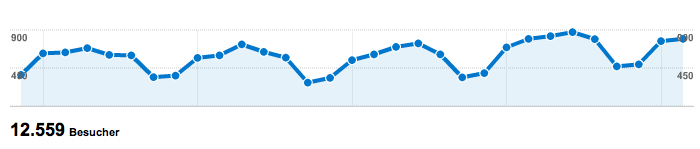
\includegraphics[width=.75\textwidth]{usage/users.png}
  \end{center}
  \caption{Besucherzahlen innerhalb eines Monats. Es ist klar ein Wochenrhythmus erkennbar.}
\end{figure}

\begin{figure}[htbp]
  \begin{center}
    \includegraphics[width=\textwidth]{usage/os.pdf}
  \end{center}
  \caption{Betriebssysteme der Nutzer}
\end{figure}

\begin{figure}[htbp]
  \begin{center}
    \includegraphics[width=\textwidth]{usage/browser.pdf}
  \end{center}
  \caption{Webbrowser der Nutzer}
\end{figure}

\begin{figure}[htbp]
  \begin{center}
    \includegraphics[width=\textwidth]{usage/country.pdf}
  \end{center}
  \caption{Länder}
\end{figure}

\begin{figure}[htbp]
  \begin{center}
    \includegraphics[width=.75\textwidth]{usage/city.pdf}
  \end{center}
  \caption{Städte}
\end{figure}

\begin{figure}[htbp]
  \begin{center}
    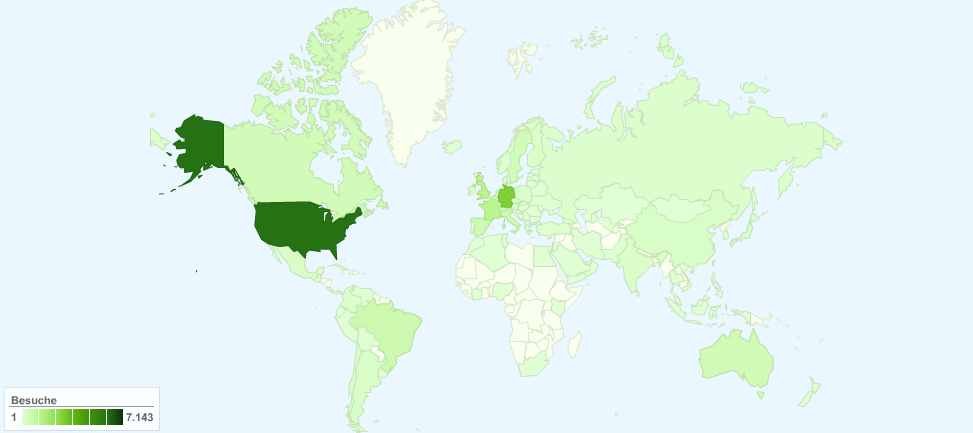
\includegraphics[width=\textwidth]{usage/countrymap.png}
  \end{center}
  \caption{Karte der Zugriffe: Länder}
\end{figure}

\begin{figure}[htbp]
  \begin{center}
    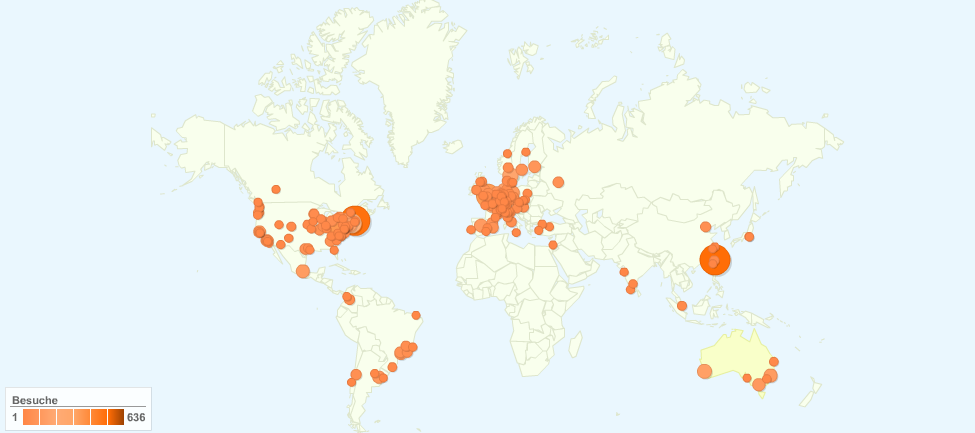
\includegraphics[width=\textwidth]{usage/citymap.png}
  \end{center}
  \caption{Karte der Zugriffe: Städte}
\end{figure}


% chapter nutzungsstatistiken (end)
